\documentclass[12pt,letterpaper]{article}
\usepackage[margin=1in]{geometry}
\usepackage{amsfonts}
\usepackage{amssymb}
\usepackage{amsthm}
\usepackage{amsmath}
\usepackage{enumerate}

%Here are some user-defined notations
\newcommand{\RR}{\mathbf R}  %bold R
\newcommand{\CC}{\mathbf C}  %bold C
\newcommand{\ZZ}{\mathbf Z}   %bold Z
\newcommand{\QQ}{\mathbf Q}   %bold Q
\newcommand{\rr}{\mathbb R}     %blackboard bold R
\newcommand{\cc}{\mathbb C}    %blackboard bold R
\newcommand{\zz}{\mathbb Z}    %blackboard bold R
\newcommand{\qq}{\mathbb Q}   %blackboard bold Q
\newcommand{\calM}{\mathcal M}  %calligraphic M
\newcommand{\sm}{\setminus} 
\newcommand{\bfa}{\mathbf a}
\newcommand{\bfb}{\mathbf b}
\newcommand{\bfc}{\mathbf c}
\newcommand{\ddx}{\dfrac{d}{dx}}


\usepackage{tikz}
\usetikzlibrary{positioning}
\usepackage{graphicx}


%Here are some user-defined operators
\newcommand{\re}{\operatorname {Re}}
\newcommand{\im}{\operatorname {Im}}


%These commands deal with theorem-like environments (i.e., italic)
\theoremstyle{plain}
\newtheorem{theorem}{Theorem}[section]
\newtheorem{corollary}[theorem]{Corollary}
\newtheorem{lemma}[theorem]{Lemma}
\newtheorem{conjecture}[theorem]{Conjecture}

%These deal with definition-like environments (i.e., non-italic)
\theoremstyle{definition}
\newtheorem{definition}[theorem]{Definition}
\newtheorem{example}[theorem]{Example}
\newtheorem{remark}[theorem]{Remark}

%your name and date in the header.
\usepackage[us]{datetime} 
\usepackage{fancyhdr}
\pagestyle{fancy}
\lhead{}
\chead{MATH 2710\\ Exam 2 questions}
\rhead{}
\lfoot{}
\cfoot{}
\rfoot{\thepage}
\renewcommand{\headrulewidth}{0 pt}
\renewcommand{\footrulewidth}{0 pt}
\begin{document}
\ \\
\begin{enumerate}[1.]
\item Prove that $a\equiv b \mod m$ is an equivalence relation. 
\ \\
\item Prove the following theorem: If $[a]$ is any non-zero element in $\mathbb{Z}_p$, where $p$ is prime, then there exists an element $[b]\in \zz_p$ such that 
\[[a]\cdot [b]=[1].\]

\ \\
\item Let $A$ be a set and define $P(A)$ to be the set of all subsets of $A$. Let $C$ be a fixed subset of the set $A$ and define relation $R$ on the set $P(A)$ by $X R Y$ if and only if $X\cap C=Y\cap C$. Prove that this is an equivalence relation. 
\ \\
\item Let $A$ be a set and let $P$ be a partition of the set $A$ i.e. $P=\{A_1, A_2, \ldots A_n\}$ where 
\begin{enumerate}[i)]
\item $A_i\subset A$, 
\item $\emptyset \not \in P$
\item $A_1\cup A_2\cup \ldots \cup A_n=A$ 
\item $A_i\cap A_j =\emptyset $ when $i\neq j$. 
\end{enumerate}
For $x,y \in A$ we say that $x R y$ if and only if $x\in A_i$ and $y\in A_i$ for the same $i$. Prove this is an equivalence relation. 
\ \\
\item Prove or disprove: The relation $R$ defined on the set $\mathbb{Z}$ by $x R y$ if and only if $xy>0$ is an equivalence relation. 
\ \\
\item A sequence of integers $x_1, x_2, x_3,\ldots $ is defined recursively by $x_1=3$, $x_2=7$ and
\[x_k=5x_{k-1}-6x_{k-2}\ \ \text{ for all }k\geq 3\]
Prove by induction that $x_n=2^n+3^{n-1}$ for all positive integers $n$. 
\ \\
\item Prove by induction that a set of $n$ elements contains $2^n$ subsets (including the set itself and $\emptyset$).
\ \\
\item Prove by induction that if $n$ points lie in a plane and no three are colinear, prove that there are $\frac{1}{2}n(n-1)$ lines joining these points. \\
\ \\
{\bf Example: }
\begin{center}

\begin{tikzpicture}
\node at (0,0){$\bullet$};
\node at (1,0){$\bullet$};
\node at (0,1){$\bullet$};
\node at (1,1){$\bullet$};
\draw (1,1)--(0,0) ;
\draw (1,0)--(0,0) ;
\draw (1,1)--(1,0) ;
\draw (0,1)--(0,0) ;
\draw (0,1)--(1,1) ;
\draw (0,1)--(1,0) ;
\end{tikzpicture}
\end{center}

\item Suppose that n chords are drawn in a circle, dividing the circle into different regions.
Prove that every region can be colored one of two colors such that adjacent regions are
different colors. \\
\ \\
{\bf Example: }
\begin{center}
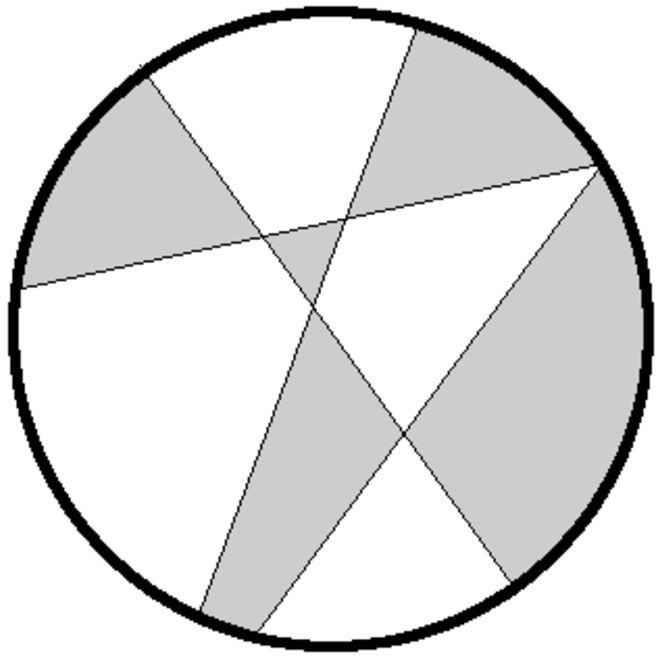
\includegraphics[scale=0.25]{circle}
\end{center}
\item Let $\phi(m):\mathbb{Z}^+\rightarrow \mathbb{Z}^+$ denote the Euler $\phi$-function. 
\[\phi(m)=\#\text{ of positive integers less or equal to } m \text{ that are relatively prime to }m\]
Prove $\phi(m)=m-1$ if and only if $m$ is prime. 
\ \\
\item Prove by induction the Leibniz rule for calculus 
\[\dfrac{d^n}{dx^n}(f\cdot g) =\sum_{r=0}^n {n \choose r} \dfrac{d^{n-r}}{dx^{n-r}}f \dfrac{d^r}{dx^r}g\]
\ \\
\item Prove that if $x\equiv 1 $ (mod 2) that 
\[x^{2^n}\equiv 1 \mod 2^{n+2} \text{ for all }n\in \mathbb{P}\]
\ \\
\item If $p$ is prime prove that 
\[(a+b)^p\equiv a^p+b^p \mod p \]
for all $a,b\in \mathbb{Z}$.
\ \\ 
\item  Prove that multiplication is a well defined operation on $\mathbb{Q}$.
\ \\
\item Prove that $\sqrt{3}$ is irrational. 
\ \\
\item If $f:X\rightarrow Y$ is a bijective function, prove that the inverse is unique. 
\ \\
\item If $f:X\rightarrow Y$ and $g:Y\rightarrow Z$ prove that 
\[(g\circ f)^{-1}=f^{-1}\circ g^{-1}\]
\ \\
\item Prove that if $A$ and $B$ are disjoint finite sets that $|A\cup B|=|A|+|B|$.
\ \\
\item Prove that $|\zz^+|=|\zz|$.
\ \\
\item Prove that $|\zz^+| \neq |\rr|$.
\ \\
\item Let $S=P(X)$ be the power set of $X$. Define the following relation on $S$: Say that $A\sim B$ if and only if $|A|=|B|$. Show that this is an equivalence relation. 
\ \\
\item Let $f:X\rightarrow X$ be a function on a finite set. Show that $f$ is injective if and only if it is surjective.
\ \\
\item Let $f:X\rightarrow Y$ and $g:Y\rightarrow Z$ be functions. Show that if $f$ and $g$ are injective that $g\circ f$ is injective. 
\ \\
\item Let $f:X\rightarrow Y$ and $g:Y\rightarrow Z$ be functions. Show that if $f$ and $g$ are surjective that $g\circ f$ is surjective. 
\ \\
\item Show that if $f:A\rightarrow P(A)$ is a function then it cannot be surjective. \\
{\bf Hint:} Let $D=\{a\in A\mid a\not\in f(a)\}$ and show that $f(a)\neq D$ for all $a\in A$.
\ \\
\end{enumerate}

\end{document}








